%!TeX root=../wowtop.tex

\ArtChapter[The Fighting Begins]{9head}

\lettrine[lines=4,findent=2pt]{S}{aturday} lives in my memory as a day of suspense. It was a day of lassitude too, hot and close, with, I am told, a rapidly fluctuating barometer. I had slept but little, though my wife had succeeded in sleeping, and I rose early. I went into my garden before breakfast and stood listening, but towards the common there was nothing stirring but a lark.

The milkman came as usual. I heard the rattle of his chariot and I went round to the side gate to ask the latest news. He told me that during the night the Martians had been surrounded by troops, and that guns were expected. Then—a familiar, reassuring note—I heard a train running towards Woking.

»They aren't to be killed,« said the milkman, »if that can possibly be avoided.«

I saw my neighbour gardening, chatted with him for a time, and then strolled in to breakfast. It was a most unexceptional morning. My neighbour was of opinion that the troops would be able to capture or to destroy the Martians during the day.

»It's a pity they make themselves so unapproachable,« he said. »It would be curious to know how they live on another planet; we might learn a thing or two.«

He came up to the fence and extended a handful of strawberries, for his gardening was as generous as it was enthusiastic. At the same time he told me of the burning of the pine woods about the Byfleet Golf Links.

»They say,« said he, »that there's another of those blessed things fallen there—number two. But one's enough, surely. This lot'll cost the insurance people a pretty penny before everything's settled.« He laughed with an air of the greatest good humour as he said this. The woods, he said, were still burning, and pointed out a haze of smoke to me. »They will be hot under foot for days, on account of the thick soil of pine needles and turf,« he said, and then grew serious over »poor Ogilvy.«

After breakfast, instead of working, I decided to walk down towards the common. Under the railway bridge I found a group of soldiers—sappers, I think, men in small round caps, dirty red jackets unbuttoned, and showing their blue shirts, dark trousers, and boots coming to the calf. They told me no one was allowed over the canal, and, looking along the road towards the bridge, I saw one of the Cardigan men standing sentinel there. I talked with these soldiers for a time; I told them of my sight of the Martians on the previous evening. None of them had seen the Martians, and they had but the vaguest ideas of them, so that they plied me with questions. They said that they did not know who had authorised the movements of the troops; their idea was that a dispute had arisen at the Horse Guards. The ordinary sapper is a great deal better educated than the common soldier, and they discussed the peculiar conditions of the possible fight with some acuteness. I described the Heat-Ray to them, and they began to argue among themselves.

»Crawl up under cover and rush 'em, say I,« said one.

»Get aht!« said another. »What's cover against this 'ere 'eat? Sticks to cook yer! What we got to do is to go as near as the ground'll let us, and then drive a trench.«

»Blow yer trenches! You always want trenches; you ought to ha' been born a rabbit Snippy.«

»Ain't they got any necks, then?« said a third, abruptly—a little, contemplative, dark man, smoking a pipe.

I repeated my description.

»Octopuses,« said he, »that's what I calls 'em. Talk about fishers of men—fighters of fish it is this time!«

»It ain't no murder killing beasts like that,« said the first speaker.

»Why not shell the darned things strite off and finish 'em?« said the little dark man. »You carn tell what they might do.«

»Where's your shells?« said the first speaker. »There ain't no time. Do it in a rush, that's my tip, and do it at once.«

So they discussed it. After a while I left them, and went on to the railway station to get as many morning papers as I could.

But I will not weary the reader with a description of that long morning and of the longer afternoon. I did not succeed in getting a glimpse of the common, for even Horsell and Chobham church towers were in the hands of the military authorities. The soldiers I addressed didn't know anything; the officers were mysterious as well as busy. I found people in the town quite secure again in the presence of the military, and I heard for the first time from Marshall, the tobacconist, that his son was among the dead on the common. The soldiers had made the people on the outskirts of Horsell lock up and leave their houses.

I got back to lunch about two, very tired for, as I have said, the day was extremely hot and dull; and in order to refresh myself I took a cold bath in the afternoon. About half past four I went up to the railway station to get an evening paper, for the morning papers had contained only a very inaccurate description of the killing of Stent, Henderson, Ogilvy, and the others. But there was little I didn't know. The Martians did not show an inch of themselves. They seemed busy in their pit, and there was a sound of hammering and an almost continuous streamer of smoke. Apparently they were busy getting ready for a struggle. »Fresh attempts have been made to signal, but without success,« was the stereotyped formula of the papers. A sapper told me it was done by a man in a ditch with a flag on a long pole. The Martians took as much notice of such advances as we should of the lowing of a cow.

I must confess the sight of all this armament, all this preparation, greatly excited me. My imagination became belligerent, and defeated the invaders in a dozen striking ways; something of my schoolboy dreams of battle and heroism came back. It hardly seemed a fair fight to me at that time. They seemed very helpless in that pit of theirs.

About three o'clock there began the thud of a gun at measured intervals from Chertsey or Addlestone. I learned that the smouldering pine wood into which the second cylinder had fallen was being shelled, in the hope of destroying that object before it opened. It was only about five, however, that a field gun reached Chobham for use against the first body of Martians.

About six in the evening, as I sat at tea with my wife in the summerhouse talking vigorously about the battle that was lowering upon us, I heard a muffled detonation from the common, and immediately after a gust of firing. Close on the heels of that came a violent rattling crash, quite close to us, that shook the ground; and, starting out upon the lawn, I saw the tops of the trees about the Oriental College burst into smoky red flame, and the tower of the little church beside it slide down into ruin. The pinnacle of the mosque had vanished, and the roof line of the college itself looked as if a hundred-ton gun had been at work upon it. One of our chimneys cracked as if a shot had hit it, flew, and a piece of it came clattering down the tiles and made a heap of broken red fragments upon the flower bed by my study window.

I and my wife stood amazed. Then I realised that the crest of Maybury Hill must be within range of the Martians' Heat-Ray now that the college was cleared out of the way.

At that I gripped my wife's arm, and without ceremony ran her out into the road. Then I fetched out the servant, telling her I would go upstairs myself for the box she was clamouring for.

»We can't possibly stay here,« I said; and as I spoke the firing reopened for a moment upon the common.

»But where are we to go?« said my wife in terror.

I thought perplexed. Then I remembered her cousins at Leatherhead.

»Leatherhead!« I shouted above the sudden noise.

She looked away from me downhill. The people were coming out of their houses, astonished.

»How are we to get to Leatherhead?« she said.

Down the hill I saw a bevy of hussars ride under the railway bridge; three galloped through the open gates of the Oriental College; two others dismounted, and began running from house to house. The sun, shining through the smoke that drove up from the tops of the trees, seemed blood red, and threw an unfamiliar lurid light upon everything.

»Stop here,« said I; »you are safe here«; and I started off at once for the Spotted Dog, for I knew the landlord had a horse and dog cart. I ran, for I perceived that in a moment everyone upon this side of the hill would be moving. I found him in his bar, quite unaware of what was going on behind his house. A man stood with his back to me, talking to him.

»I must have a pound,« said the landlord, »and I've no one to drive it.«

»I'll give you two,« said I, over the stranger's shoulder.

»What for?«

»And I'll bring it back by midnight,« I said.

»Lord!« said the landlord; »what's the hurry? I'm selling my bit of a pig. Two pounds, and you bring it back? What's going on now?«

I explained hastily that I had to leave my home, and so secured the dog cart. At the time it did not seem to me nearly so urgent that the landlord should leave his. I took care to have the cart there and then, drove it off down the road, and, leaving it in charge of my wife and servant, rushed into my house and packed a few valuables, such plate as we had, and so forth. The beech trees below the house were burning while I did this, and the palings up the road glowed red. While I was occupied in this way, one of the dismounted hussars came running up. He was going from house to house, warning people to leave. He was going on as I came out of my front door, lugging my treasures, done up in a tablecloth. I shouted after him:

»What news?«

He turned, stared, bawled something about »crawling out in a thing like a dish cover,« and ran on to the gate of the house at the crest. A sudden whirl of black smoke driving across the road hid him for a moment. I ran to my neighbour's door and rapped to satisfy myself of what I already knew, that his wife had gone to London with him and had locked up their house. I went in again, according to my promise, to get my servant's box, lugged it out, clapped it beside her on the tail of the dog cart, and then caught the reins and jumped up into the driver's seat beside my wife. In another moment we were clear of the smoke and noise, and spanking down the opposite slope of Maybury Hill towards Old Woking.

In front was a quiet sunny landscape, a wheat field ahead on either side of the road, and the Maybury Inn with its swinging sign. I saw the doctor's cart ahead of me. At the bottom of the hill I turned my head to look at the hillside I was leaving. Thick streamers of black smoke shot with threads of red fire were driving up into the still air, and throwing dark shadows upon the green treetops eastward. The smoke already extended far away to the east and west—to the Byfleet pine woods eastward, and to Woking on the west. The road was dotted with people running towards us. And very faint now, but very distinct through the hot, quiet air, one heard the whirr of a machine-gun that was presently stilled, and an intermittent cracking of rifles. Apparently the Martians were setting fire to everything within range of their Heat-Ray.

I am not an expert driver, and I had immediately to turn my attention to the horse. When I looked back again the second hill had hidden the black smoke. I slashed the horse with the whip, and gave him a loose rein until Woking and Send lay between us and that quivering tumult. I overtook and passed the doctor between Woking and Send.

\begin{figure}[b!]
\centering
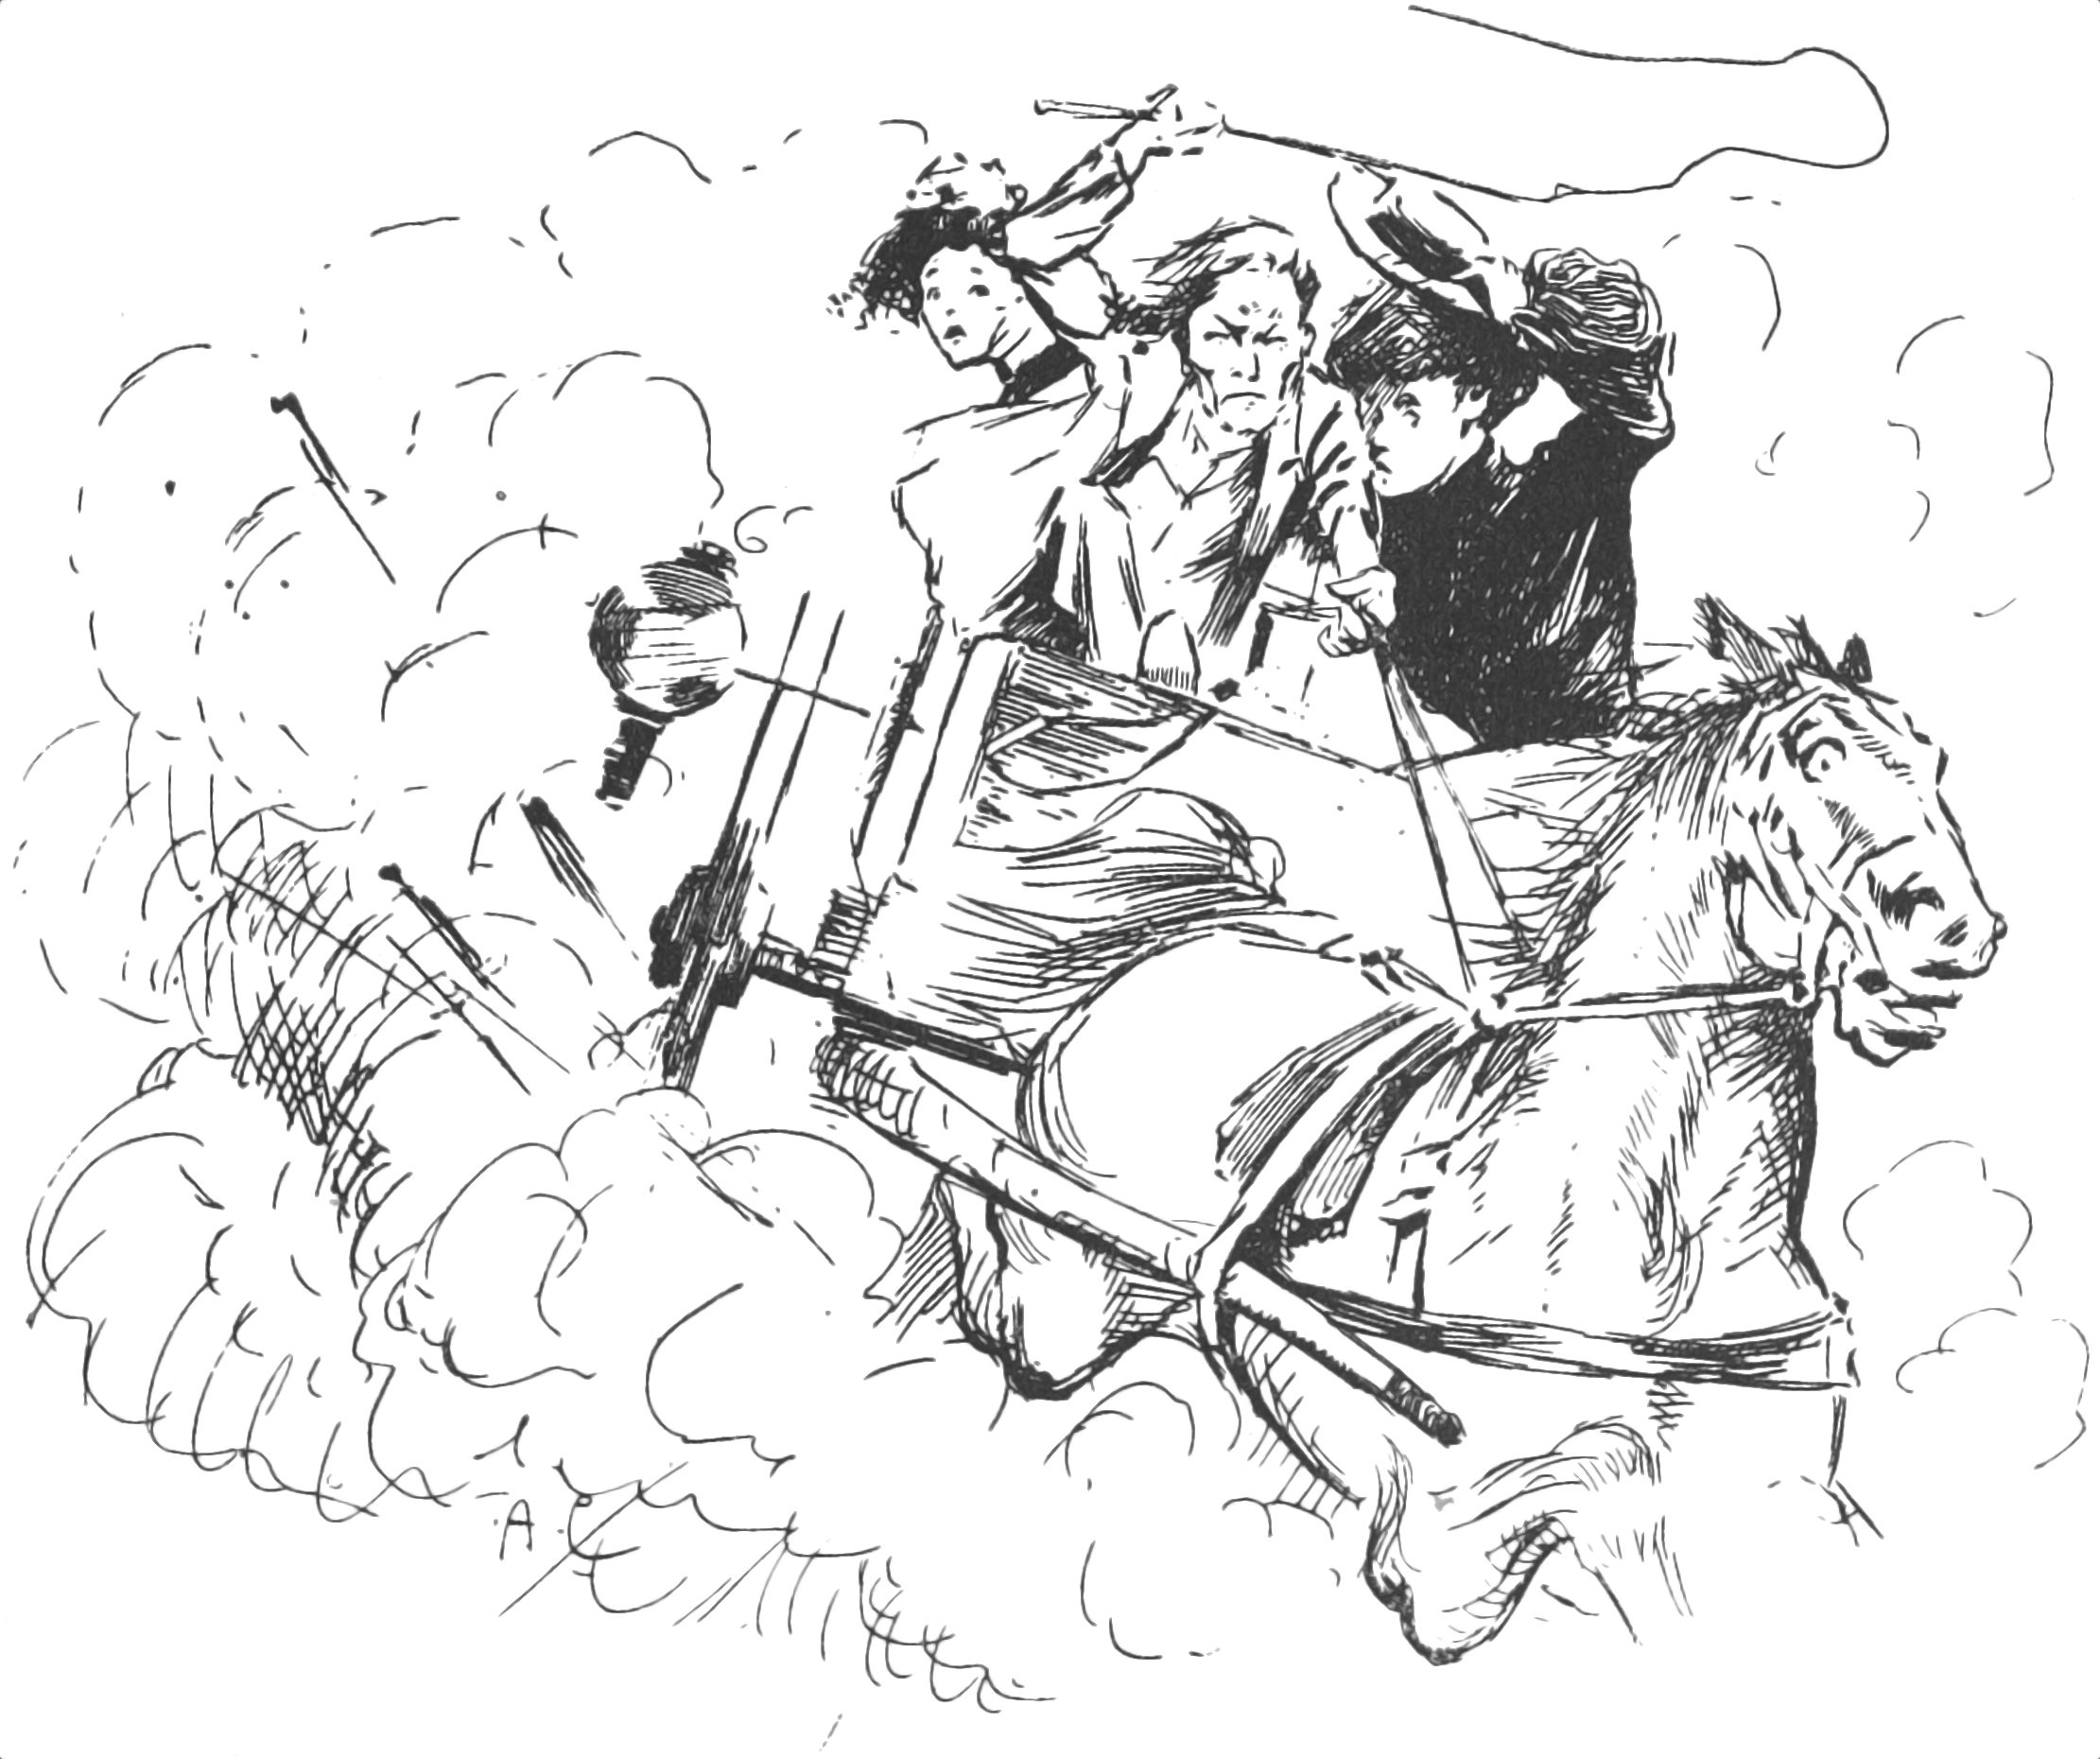
\includegraphics[width=\tailpiecesize]{9tailpiece}
%\captionlistentry{Tailpiece to Chapter \thechapter}
\end{figure}

